%% abtex2-modelo-artigo.tex, v-1.9.6 laurocesar
%% Copyright 2012-2016 by abnTeX2 group at http://www.abntex.net.br/ 
%%
%% This work may be distributed and/or modified under the
%% conditions of the LaTeX Project Public License, either version 1.3
%% of this license or (at your option) any later version.
%% The latest version of this license is in
%%   http://www.latex-project.org/lppl.txt
%% and version 1.3 or later is part of all distributions of LaTeX
%% version 2005/12/01 or later.
%%
%% This work has the LPPL maintenance status `maintained'.
%% 
%% The Current Maintainer of this work is the abnTeX2 team, led
%% by Lauro César Araujo. Further information are available on 
%% http://www.abntex.net.br/
%%
%% This work consists of the files abntex2-modelo-artigo.tex and
%% abntex2-modelo-references.bib
%%

% ------------------------------------------------------------------------
% ------------------------------------------------------------------------
% abnTeX2: Modelo de Artigo Acadêmico em conformidade com
% ABNT NBR 6022:2003: Informação e documentação - Artigo em publicação 
% periódica científica impressa - Apresentação
% ------------------------------------------------------------------------
% ------------------------------------------------------------------------

\documentclass[
	% -- opções da classe memoir --
	article,			% indica que é um artigo acadêmico
	11pt,				% tamanho da fonte
	oneside,			% para impressão apenas no recto. Oposto a twoside
	a4paper,			% tamanho do papel. 
	% -- opções da classe abntex2 --
	%chapter=TITLE,		% títulos de capítulos convertidos em letras maiúsculas
	%section=TITLE,		% títulos de seções convertidos em letras maiúsculas
	%subsection=TITLE,	% títulos de subseções convertidos em letras maiúsculas
	%subsubsection=TITLE % títulos de subsubseções convertidos em letras maiúsculas
	% -- opções do pacote babel --
	english,			% idioma adicional para hifenização
	brazil,				% o último idioma é o principal do documento
	sumario=tradicional
	]{abntex2}


% ---
% PACOTES
% ---

% ---
% Pacotes fundamentais 
% ---
\usepackage{lmodern}			% Usa a fonte Latin Modern
\usepackage[T1]{fontenc}		% Selecao de codigos de fonte.
\usepackage[utf8]{inputenc}		% Codificacao do documento (conversão automática dos acentos)
\usepackage{indentfirst}		% Indenta o primeiro parágrafo de cada seção.
\usepackage{nomencl} 			% Lista de simbolos
\usepackage{color}				% Controle das cores
\usepackage{graphicx}			% Inclusão de gráficos
\usepackage{microtype} 			% para melhorias de justificação
\usepackage{listings}			% Para código-fonte
% ---
\usepackage{multirow}
\usepackage{enumitem}
\setlist[description]{leftmargin=\parindent,labelindent=\parindent}
\renewcommand{\lstlistingname}{Exemplo}
\graphicspath{ {img/} }
		
% ---
% Pacotes adicionais, usados apenas no âmbito do Modelo Canônico do abnteX2
% ---
\usepackage{lipsum}				% para geração de dummy text
% ---
		
% ---
% Pacotes de citações
% ---
\usepackage[brazilian,hyperpageref]{backref}	 % Paginas com as citações na bibl
\usepackage[alf]{abntex2cite}	% Citações padrão ABNT
% ---

% ---
% Configurações do pacote backref
% Usado sem a opção hyperpageref de backref
\renewcommand{\backrefpagesname}{Citado na(s) página(s):~}
% Texto padrão antes do número das páginas
\renewcommand{\backref}{}
% Define os textos da citação
\renewcommand*{\backrefalt}[4]{
	\ifcase #1 %
		Nenhuma citação no texto.%
	\or
		Citado na página #2.%
	\else
		Citado #1 vezes nas páginas #2.%
	\fi}%
% ---

% ---
% Informações de dados para CAPA e FOLHA DE ROSTO
% ---
\titulo{GPX - Implementação}
\autor{Ozéas Quevedo de Carvalho\thanks{Aluno Regular - PPGI - RA 1801562} \and
	Prof. Dr. Danilo Sipoli Sanches}
\local{Brasil}
\data{17 de setembro de 2018}
% ---

% ---
% Configurações de aparência do PDF final

% alterando o aspecto da cor azul
\definecolor{blue}{RGB}{41,5,195}

% informações do PDF
\makeatletter
\hypersetup{
     	%pagebackref=true,
		pdftitle={\@title}, 
		pdfauthor={\@author},
    	pdfsubject={Modelo de artigo científico com abnTeX2},
	    pdfcreator={LaTeX with abnTeX2},
		pdfkeywords={abnt}{latex}{abntex}{abntex2}{atigo científico}, 
		colorlinks=true,       		% false: boxed links; true: colored links
    	linkcolor=blue,          	% color of internal links
    	citecolor=blue,        		% color of links to bibliography
    	filecolor=magenta,      		% color of file links
		urlcolor=blue,
		bookmarksdepth=4
}
\makeatother
% --- 

% ---
% compila o indice
% ---
\makeindex
% ---

% ---
% Altera as margens padrões
% ---
\setlrmarginsandblock{3cm}{3cm}{*}
\setulmarginsandblock{3cm}{3cm}{*}
\checkandfixthelayout
% ---

% --- 
% Espaçamentos entre linhas e parágrafos 
% --- 

% O tamanho do parágrafo é dado por:
\setlength{\parindent}{1.3cm}

% Controle do espaçamento entre um parágrafo e outro:
\setlength{\parskip}{0.2cm}  % tente também \onelineskip

% Espaçamento simples
\SingleSpacing

% ----
% Início do documento
% ----
\begin{document}

% Seleciona o idioma do documento (conforme pacotes do babel)
%\selectlanguage{english}
\selectlanguage{brazil}

% Retira espaço extra obsoleto entre as frases.
\frenchspacing 

% ----------------------------------------------------------
% ELEMENTOS PRÉ-TEXTUAIS
% ----------------------------------------------------------

%---
%
% Se desejar escrever o artigo em duas colunas, descomente a linha abaixo
% e a linha com o texto ``FIM DE ARTIGO EM DUAS COLUNAS''.
% \twocolumn[    		% INICIO DE ARTIGO EM DUAS COLUNAS
%
%---
% página de titulo
\maketitle

% ]  				% FIM DE ARTIGO EM DUAS COLUNAS
% ---

% ----------------------------------------------------------
% ELEMENTOS TEXTUAIS
% ----------------------------------------------------------
\textual

% ----------------------------------------------------------
% Introdução
% ----------------------------------------------------------
\section{Partições Factíveis e não-Factíveis}

De acordo com \citeonline{Tinos2014}, para ser factível, uma partição deve ter o mesmo grafo simplificado para ambas soluções. O grafo simplificado é construído substituindo o caminho entre o vértice de entrada e saída dentro da partição por um único vértice. A Figura \ref{fig-1}, retirada do mesmo trabalho, contém um exemplo da construção do grafo simplificado. Nesse caso, ambas as partições são factíveis para combinação, já que cada partição apresenta o mesmo grafo simplificado para cada solução. As partições que não passam no teste do grafo simplificado são consideradas não factíveis e são encaminhadas para a etapa de fusão.

\begin{figure}[tbph!]
	\centering
	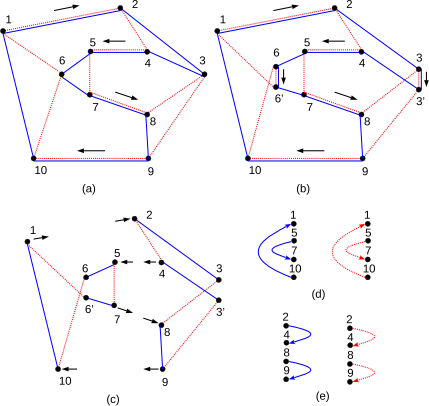
\includegraphics[width=0.7\linewidth]{fig-1}
	\caption{\citeonline{Tinos2014}, Figura 3.}
	\label{fig-1}
\end{figure}

A Figura \ref{fig-2}, retirada do artigo \citeonline{Tinos2018b}, contém 6 partições obtidas após os cortes de arestas duplas. Evidentemente, por possuírem apenas uma entrada e saída, as partições A e B são factíveis. No entanto, de acordo com o artigo, os grafos simplificados das demais partições não são iguais para cada solução pai, portanto são infactíveis.

\begin{figure}[tbph!]
	\centering
	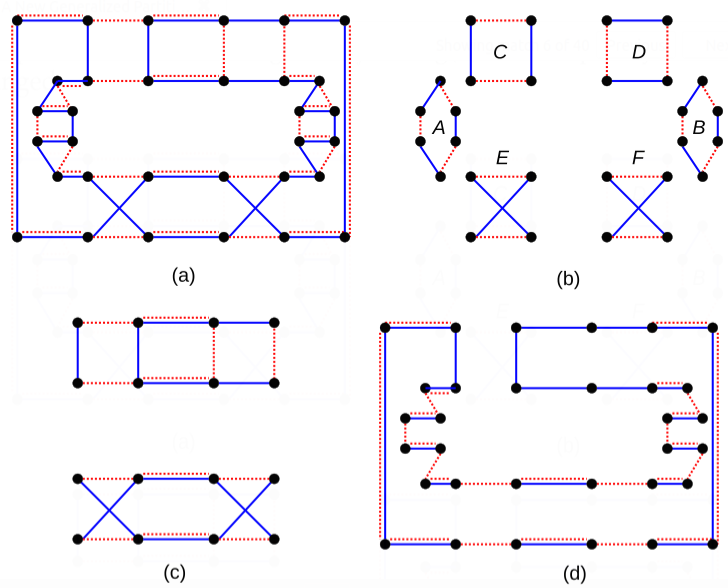
\includegraphics[width=0.7\linewidth]{fig-2}
	\caption{\citeonline{Tinos2018b}, Figura 5.}
	\label{fig-2}
\end{figure}

% Please add the following required packages to your document preamble:
% \usepackage[normalem]{ulem}
% \useunder{\uline}{\ul}{}
\begin{table}[tbph!]
	\centering
	\label{tab-1}
	\begin{tabular}{ccc}
		Partição & Solução & Grafo Simplificado \\
		A & Azul & 4: 9 \\
		A & Vermelha & 4: 9 \\
		B & Azul & 14: 19 \\
		B & Vermelha & 14: 19 \\
		C & Azul & 2: 3, 22: 23 \\
		C & Vermelha & 2: 23, 22: 3 \\
		D & Azul & 24: 25, 20: 21 \\
		D & Vermelha & 24: 21, 20: 25 \\
		E & Azul & 10: 11, 30: 31 \\
		E & Vermelha & 10: 30, 11: 31 \\
		F & Azul & 28: 29, 12: 13 \\
		F & Vermelha & 28: 12, 29: 13
	\end{tabular}
\end{table}

De acordo com a nomeação de vértices da Figura \ref{fig-3}, temos os grafos simplificados apresentados na Tabela \ref{tab-1}. Com efeito, como podemos ver na Figura \ref{fig-3}, caso se escolha o percurso azul na partição C e o percurso vermelho na partição D, o percurso final não forma um ciclo hamiltoniano, independente das escolhas nas demais partições.

\begin{figure}[tbph!]
	\centering
	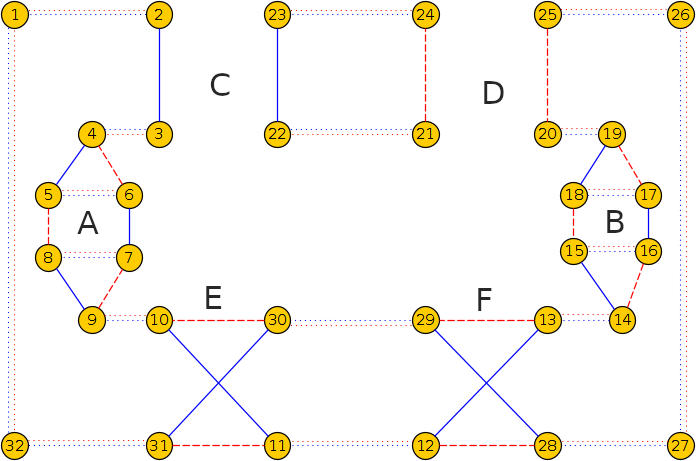
\includegraphics[width=0.7\linewidth]{fig-3}
	\caption{Azul na partição C e vermelho na partição D não resulta em ciclo hamiltoniano.}
	\label{fig-3}
\end{figure}

Podemos observar, no entanto, que independente das escolhas de cor nas partições E e F, caso se escolha uma mesma cor nas partições C e D (fusão), um ciclo hamiltoniano é formado, como podemos ver nas Figuras \ref{fig-4} e \ref{fig-5}.

\begin{figure}[tbph!]
	\centering
	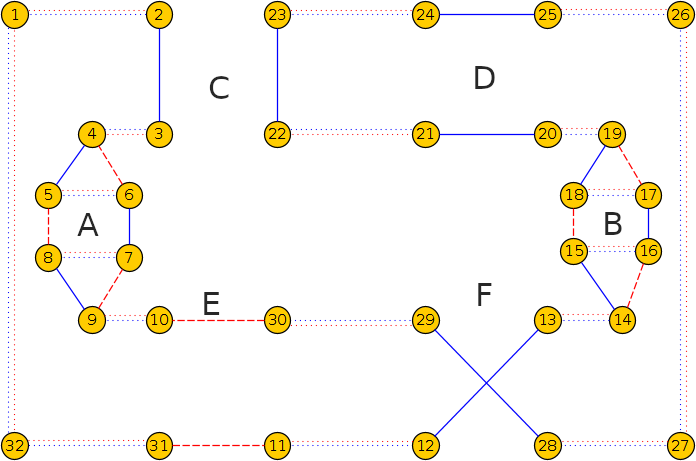
\includegraphics[width=0.7\linewidth]{fig-4}
	\caption{Vermelho na E e Azul na F resulta em recombinação válida. C e D com mesma cor.}
	\label{fig-4}
\end{figure}

\begin{figure}[tbph!]
	\centering
	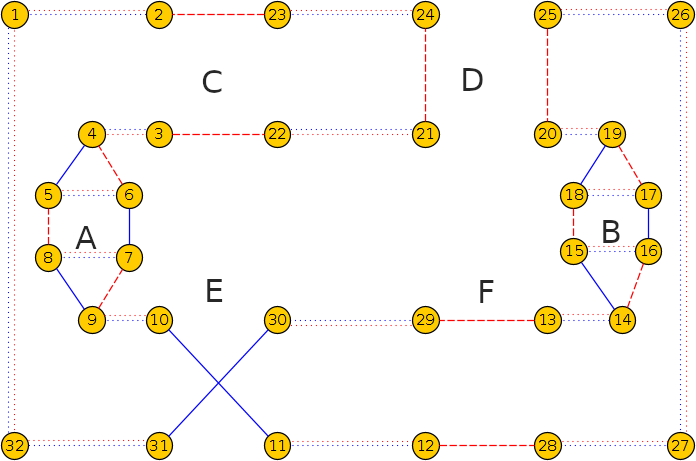
\includegraphics[width=0.7\linewidth]{fig-5}
	\caption{Azul na E e Vermelho na F resulta em recombinação válida. C e D com mesma cor.}
	\label{fig-5}
\end{figure}

Com base nessas observações, formulamos um teste de factibilidade adicional com a intenção de ampliar a capacidade do GPX em identificar partições válidas para a recombinação, diminuindo estatisticamente, em consequência, a quantidade de partições inválidas testadas na etapa de fusão. A Figura \ref{fig-6} apresenta quatro partições válidas que não passam no teste do grafo simplificado, mas passam no teste adicional. As figuras \ref{fig-7} e \ref{fig-8} apresentam duas soluções geradas pela combinação de diferentes cores em cada partição. A Tabela \ref{fig-2} apresenta os respectivos grafos simplificados. Como podemos ver, nenhuma dessas partições passa no teste do grafo simplificado, mas passa no teste adicional criado.

\begin{figure}[tbph!]
	\centering
	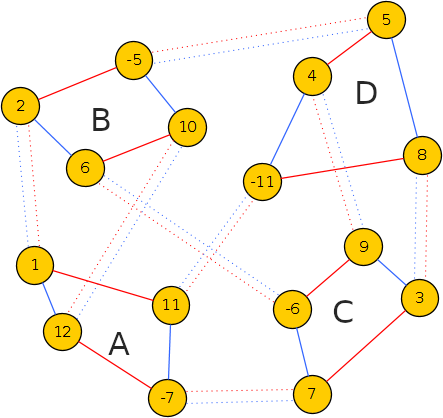
\includegraphics[width=0.5\linewidth]{fig-6}
	\caption{Quatro partições válidas}
	\label{fig-6}
\end{figure}

\begin{figure}[tbph!]
	\centering
	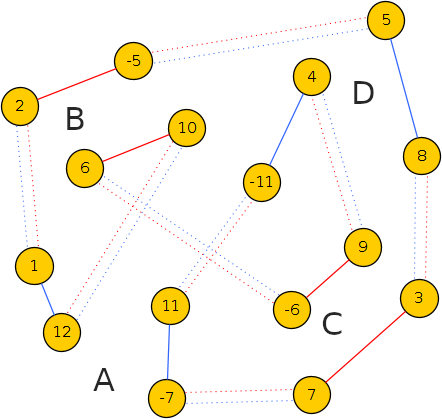
\includegraphics[width=0.5\linewidth]{fig-7}
	\caption{Possível solução por escolhas de diferentes cores em cada partição}
	\label{fig-7}
\end{figure}

\begin{figure}[tbph!]
	\centering
	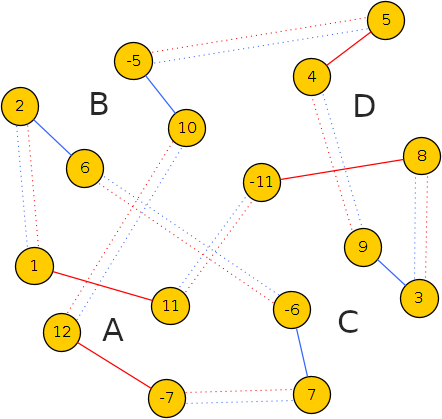
\includegraphics[width=0.5\linewidth]{fig-8}
	\caption{Possível solução por escolhas de diferentes cores em cada partição}
	\label{fig-8}
\end{figure}

% Please add the following required packages to your document preamble:
% \usepackage[normalem]{ulem}
% \useunder{\uline}{\ul}{}
\begin{table}[tbph!]
	\label{tab-2}
	\centering
	\begin{tabular}{ccc}
		Partição & Solução & Grafo Simplificado \\
		A & Azul & -7: 11, 12: 1 \\
		A & Vermelha & 11: 1, 12: -7 \\
		B & Azul & 2: 6, -5: 10 \\
		B & Vermelha & 2: -5, 6: 10 \\
		C & Azul & 9: 3, -6: 7 \\
		C & Vermelha & 9: -6, 7: 3 \\
		D & Azul & 8: 5, -11: 4 \\
		D & Vermelha & 8: -11, 5: 4
	\end{tabular}
\end{table}

Porém, após uma amostragem de soluções geradas aleatoriamente, encontramos partições inválidas que passam no segundo teste formulado, indicando a necessidade de uma reformulação do teste, ponto atual de nossa investigação.











\pagebreak
% ---
% Finaliza a parte no bookmark do PDF, para que se inicie o bookmark na raiz
% ---
\bookmarksetup{startatroot}% 
% ---


% ----------------------------------------------------------
% ELEMENTOS PÓS-TEXTUAIS
% ----------------------------------------------------------
\postextual



% ----------------------------------------------------------
% Referências bibliográficas
% ----------------------------------------------------------
\bibliography{/home/ozeas/Dropbox/Projetos/bibtex/library}


\end{document}
